\documentclass[a4paper,11pt,twoside,titlepage,openright]{book}

\usepackage[english]{babel}
\usepackage{color}
\usepackage{graphicx}
\usepackage{amsmath}
\numberwithin{equation}{section}
\usepackage[margin=3cm]{geometry}
\usepackage{hyperref}
\pagestyle{plain}

\newcommand{\ud}[1]{\underline{#1}}
\newcommand{\lt}{\left}
\newcommand{\rt}{\right}
\DeclareMathOperator{\e0}{\epsilon_0}
\newcommand{\wdg}{\wedge}
\newcommand{\emis}{\emph{emissivity}}
\newcommand{\ema}{\epsilon^{\eta}}
\newcommand{\hypot}[1]{\textbf{\textcolor{green}{#1}}}


\begin{document}

\title{Optimizing the coputation of LOS PIn / POut for a toroidal vessel} 
\author{Didier VEZINET}
\date{26.06.2017}
\maketitle

\tableofcontents

\chapter{Definitions}

Let's consider a orthonormal direct cylindrical coordinate system $(O,\ud{e}_R,\ud{e}_{\theta},\ud{e}_Z)$ associated to the orthonormal direct cartesian coordinate system $(O,\ud{e}_X,\ud{e}_Y,\ud{e}_Z)$.
Let's consider a fraction of a cone $C$ defined by a segment in $(R,Z)$ coordinates: $\ud{A}=\left(\begin{array}{cc}R_A\\Z_A\end{array}\right)$ and $\ud{B}=\left(\begin{array}{cc}R_B\\Z_B\end{array}\right)$, associated to the normalized directing vector $\ud{v}=\frac{\ud{AB}}{\|\ud{AB}\|}$ of coordinates $(v_R,v_Z)$.
We assume that $A\neq B$, so they can't have identical coordinates.


Then, any point $M$ with coordinates $(X,Y,Z)$ or $(R,\theta,Z)$ belongs to the fragment of cone $C$ defined by $A$ and $B$ if and only if:
$$
\exists q \in [0;1] / 
\left\{ \begin{array}{ll}
R-R_A = q(R_B-R_A)\\
Z-Z_A = q(Z_B-Z_A)
\end{array}\right.
$$


Now let's consider a LOS $L$ (i.e.: a half-infinite line) defined by a point $D$ and a normalized directing vector $u$, of respective coordinates $(X_D,Y_D,Z_D)$ or $(R_D,\theta_D,Z_D)$ and $(u_X,u_Y,u_Z)$.
Then, point M belongs to $L$ if and only if:
$$
\exists k \in [0;\infty[ / \ud{DM} = k\ud{u}
$$


\chapter{Derivation}

Let us now consider all intersections between cone $C$ and semi-line $L$.

$$
\begin{array}{lll}
\exists (q,k) \in [0;1]\times [0;\infty[ /& & 
\left\{\begin{array}{ll}
R-R_A = q(R_B-R_A)\\
Z-Z_A = q(Z_B-Z_A)\\
X-X_D = ku_X\\
Y-Y_D = ku_Y\\
Z-Z_D = ku_Z
\end{array}\right.\\
\end{array}
$$

Which yields (by combining to keep only unknowns $q$ and $k$):
$$
\begin{array}{cc}
q(Z_B-Z_A) = Z_D-Z_A + ku_Z\\
q^2(R_B-R_A)^2 + 2qR_A(R_B-R_A) = \left(k\ud{u}_{//} + \ud{D}_{//}\right)^2 - R_A^2
\end{array}
$$

Where we have introduced $R_D = \sqrt{X_D^2+Y_D^2}$, $\ud{u}_{//} = u_X\ud{e}_X+u_Y\ud{e}_Y$ and $\ud{D}_{//} = X_D\ud{e}_X + Y_D\ud{e}_Y$.
We can then derive a decision tree.


Given that the parallelization will take place on the LOS (i.e.: not on the cones which are parts of the vacuum vessel), we will discriminate case based prioritarily on the components of $\ud{u}$ and $D$.
We will detail only the cases which have solutions, in order to make it as clear as possible for implementation of an efficient algorithm.
We will also only consider non-tangential solution, as we are looking for entry/exit points.

\section{$u_Z=0$: horizontal LOS}

Then:
$$
\begin{array}{lll}
\exists (q,k) \in [0;1]\times [0;\infty[ /& &
\left\{\begin{array}{ll}
R-R_A = q(R_B-R_A)\\
Z_D-Z_A = q(Z_B-Z_A)\\
X-X_D = ku_X\\
Y-Y_D = ku_Y\\
Z=Z_D
\end{array}\right.\\
\end{array}
$$

If $Z_B=Z_A$ (the cone is horizontal too) and:
\begin{itemize}
\item $Z_D=Z_A \Rightarrow$ the cone stands in the same plane as the LOS $\Rightarrow$ infinity of solutions, we consider no solutions as this is a limit case with no clearly identified intersection.
\item $Z_D\neq Z_A \Rightarrow$ the cone and the LOS stand in different parallel planes $\Rightarrow$ no solution.
\end{itemize}

Hence, the only derivable solutions suppose that $Z_B\neq Z_A$.

\subsection{$Z_B\neq Z_A$ (non-horizontal cone)}

Then $q=\frac{Z_D-Z_A}{Z_B-Z_A}$.
There are acceptable solution only if $q\in[0;1]$.
By introducing $C = q^2(R_B-R_A)^2 + 2qR_A(R_B-R_A) + R_A^2$, we have:
$$
\left(k\ud{u}_{//} + \ud{D}_{//}\right)^2 - C = 0\\
\Leftrightarrow k^2\ud{u}_{//}^2 + 2k\ud{u}_{//}\cdot\ud{D}_{//} + \ud{D}_{//}^2-C = 0
$$

Then introducing $\Delta = 4\left(\ud{u}_{//}\cdot\ud{D}_{//}\right)^2 - 4\ud{u}_{//}^2\left(\ud{D}_{//}^2-C\right) = 4\delta$, there are non-tangential solutions only if $\left(\ud{u}_{//}\cdot\ud{D}_{//}\right)^2 > \ud{u}_{//}^2\left(\ud{D}_{//}^2-C\right)$.
It is necessary to compute the solutions k because we need to check if $k>=0$.

$$
k_{1,2} = \frac{-\ud{u}_{//}\cdot\ud{D}_{//} \pm \sqrt{\delta}}{\ud{u}_{//}^2}
$$

Hence, we have solutions if:
$$
\left\{
\begin{array}{lll}
u_Z = 0\\
Z_B\neq Z_A\\
\frac{Z_D-Z_A}{Z_B-Z_A} \in [0;1]\\
k_{1,2} = \frac{-\ud{u}_{//}\cdot\ud{D}_{//} \pm \sqrt{\delta}}{\ud{u}_{//}^2} \geq 0
\end{array}
\right.
$$

\section{$u_Z\neq0$: non-horizontal LOS}

Then $k=q\frac{Z_B-Z_A}{u_Z} - \frac{Z_D-Z_A}{u_Z}$, which means:


$$
\begin{array}{lll}
& q^2(R_B-R_A)^2 + 2qR_A(R_B-R_A) + R_A^2\\
= &\left(\left(q\frac{Z_B-Z_A}{u_Z} - \frac{Z_D-Z_A}{u_Z}\right)\ud{u}_{//} + \ud{D}_{//}\right)^2\\
= &\left(q\frac{Z_B-Z_A}{u_Z} - \frac{Z_D-Z_A}{u_Z}\right)^2\ud{u}_{//}^2 + 2\left(q\frac{Z_B-Z_A}{u_Z} - \frac{Z_D-Z_A}{u_Z}\right)\ud{u}_{//}\cdot\ud{D}_{//} + \ud{D}_{//}^2\\
= &q^2\left(\frac{Z_B-Z_A}{u_Z}\right)^2\ud{u}_{//}^2 - 2q\frac{Z_B-Z_A}{u_Z}\frac{Z_D-Z_A}{u_Z}\ud{u}_{//}^2 + \left(\frac{Z_D-Z_A}{u_Z}\right)^2\ud{u}_{//}^2
+ 2q\frac{Z_B-Z_A}{u_Z}\ud{u}_{//}\cdot\ud{D}_{//} - 2\frac{Z_D-Z_A}{u_Z}\ud{u}_{//}\cdot\ud{D}_{//} + \ud{D}_{//}^2\\ 
\end{array}
$$

Hence:
$$
\begin{array}{lll}
0 = && q^2\left( (R_B-R_A)^2 - \left(\frac{Z_B-Z_A}{u_Z}\right)^2\ud{u}_{//}^2 \right)\\
& + & 2q\left( R_A(R_B-R_A) + \frac{Z_B-Z_A}{u_Z}\frac{Z_D-Z_A}{u_Z}\ud{u}_{//}^2 - \frac{Z_B-Z_A}{u_Z}\ud{u}_{//}\cdot\ud{D}_{//}  \right)\\
& - & \left(\frac{Z_D-Z_A}{u_Z}\right)^2\ud{u}_{//}^2 + 2\frac{Z_D-Z_A}{u_Z}\ud{u}_{//}\cdot\ud{D}_{//} - \ud{D}_{//}^2 + R_A^2 
\end{array}
$$

We can then introduce:
$$
\left\{
\begin{array}{ll}
A = (R_B-R_A)^2 - \left(\frac{Z_B-Z_A}{u_Z}\right)^2\ud{u}_{//}^2\\
B = R_A(R_B-R_A) + \frac{Z_B-Z_A}{u_Z}\frac{Z_D-Z_A}{u_Z}\ud{u}_{//}^2 - \frac{Z_B-Z_A}{u_Z}\ud{u}_{//}\cdot\ud{D}_{//}\\
C = -\left(\frac{Z_D-Z_A}{u_Z}\right)^2\ud{u}_{//}^2 + 2\frac{Z_D-Z_A}{u_Z}\ud{u}_{//}\cdot\ud{D}_{//} - \ud{D}_{//}^2 + R_A^2
\end{array}
\right.
$$

Because of the shape of potential solutions, we have to discriminate the case $A=0$.

\subsection{$A=0$: LOS parallel to one of the cone generatrices}

Then, because of the shape of the potential solution, we have to discriminate the case $B=0$.
But in this case we have $C=0$. 
\begin{itemize}
\item if $C=0 \Rightarrow$ no condition on q and k, the LOS is included in the cone $\Rightarrow$ we consider no solution
\item if $C\neq 0 \Rightarrow$ Impossible, no solution
\end{itemize}

Only the case $B\neq 0$ is thus relevant.

\subsubsection{$B\neq0$: LOS not included in the cone}

Then, there is either one or no solution:
$$
\left\{
\begin{array}{ll}
q = -\frac{C}{2B} & \in [0,1]\\
k = q\frac{Z_B-Z_A}{u_Z} - \frac{Z_D-Z_A}{u_Z} & \geq 0
\end{array}
\right.
$$

\subsection{$A\neq 0$: LOS not parallel to a cone generatrix}

Then, we only consider cases with two distinct solutions (i.e.: no tangential case):
$$
\left\{
\begin{array}{ll}
B^2 > AC\\
q = \frac{-B \pm \sqrt{B^2-AC}}{A} & \in [0,1]\\
k = q\frac{Z_B-Z_A}{u_Z} - \frac{Z_D-Z_A}{u_Z} & \geq 0
\end{array}
\right.
$$



\chapter{Results}

\section{Upgrades}

The algorithm originally implemented in ToFu (hereafter called 'original') resorted to two nested \textbf{for} loops in Cython (i.e.: in the General\_Geom\_cy.pyx file). 
For each semi-line, a \textbf{for} loop was run on all the segments consistuting the POly of the provided vessel.
In addition to being slow (despite Cython), this 'original' algorithm seemed to return wrong results in some particular cases, due to the fact it had been written in haste and the analytical derivations had not been preserved.

This Note thus includes a full analytical derivation of the formulas to be used, as these formulas are implemented in ToFu in matricial form.

Indeed, using the above derivations, an intermediate algorithm replacing the inner \textbf{for} loop (i.e.: the loop on the segments) bya matricial computation is first created. It is called 'Inter' and is used as an intermediate test-bench to make sure it is faster and returns correct results by benchmarking against 'original', including in the identified problematic cases.

This intermediate check being conclusive, a fully matricial algorithm is derived, handling the coputation of PIn and POut for N LOS with a vessel with Ns segments, called 'Multi', thus getting rid of both \textbf{for} loops.
That new algorithm is successfully tested, and a last version is derived using only flattened arrays and avoiding redundant declarartions of large arrays, to access an ultimate speed gain? That last algorithm is called 'Multi\_Flat'.*

The figure below shows a benchmark on CEA/IRFM/spica of all algorithms ('original', 'Interm', 'Multi' and 'Multi\_Flat'), for a several values of N (number of LOS) and several values of Ns (number of segments).
Knowing that a typical vessel includes between 50 and 100 segments, and that for a single detector we usually define several tens of thousands of LOS, we can reasonably assume the total speed gain between 'original' and 'Multi\_Flat' is typically of the order of .

That upgrade is new in ToFu v.

\begin{figure}
  \caption{Benchmark of available algorithms for the computation of PIn / POut for N LOS with a vessel constituted of Ns segments. CPU time is in seconds.}
  \centering
    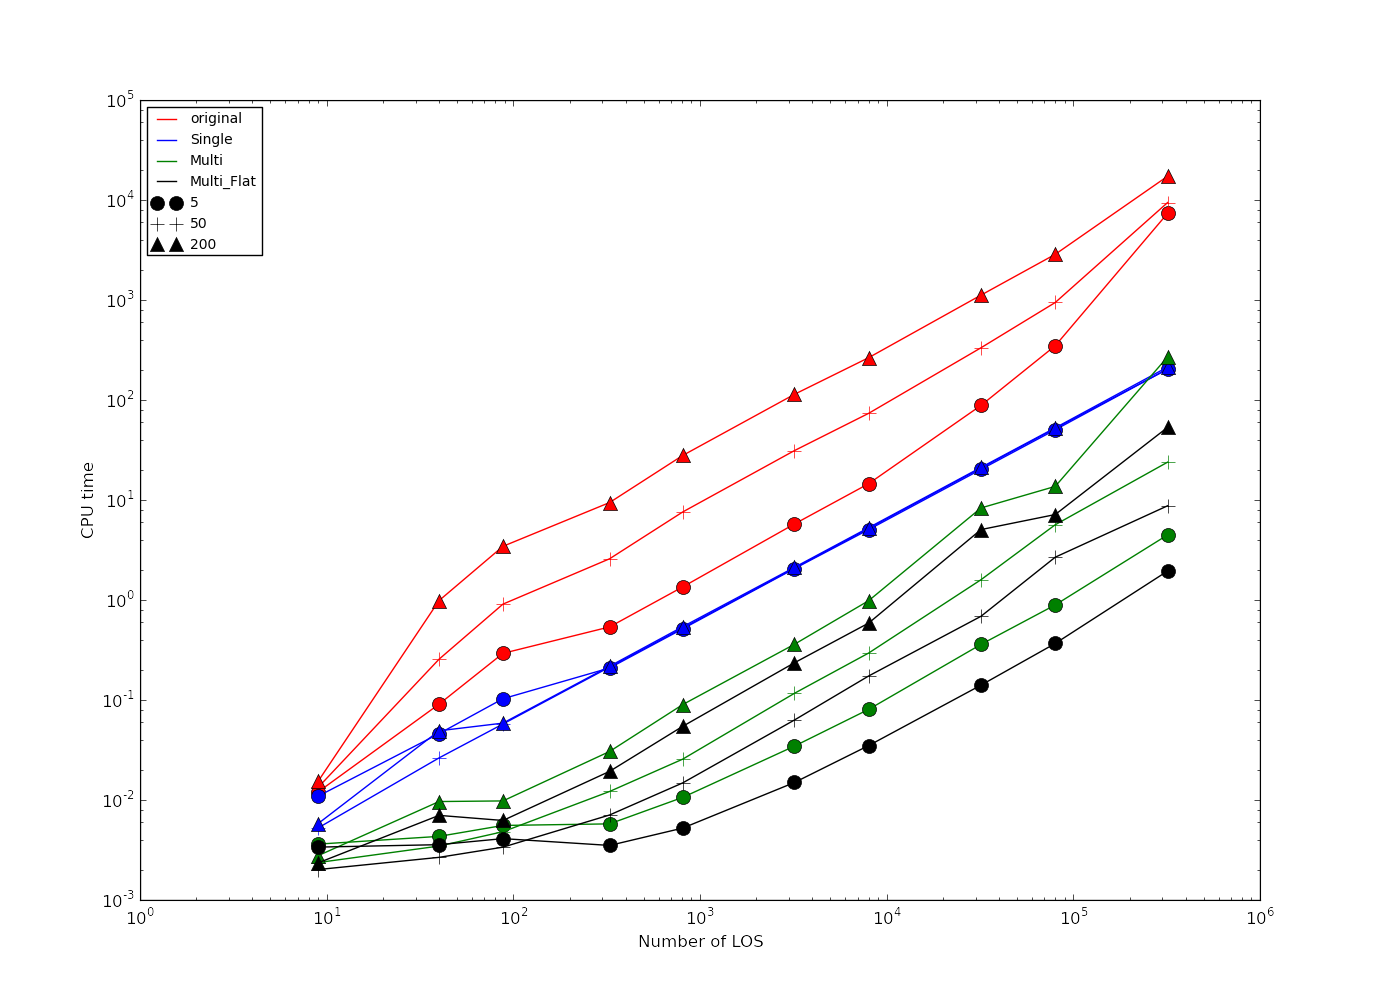
\includegraphics[width=1.\textwidth]{Fig_Stats_Timing_Ref.png}
\end{figure}

A test on one of the detectors of the WEST.Bolo diagnostic yielded the following results: computing Detect.\_set\_SinoSpan() took on average 5.7 s with 'Multi\_Flat' and 6 min 14 s with 'original', resulting in a speed improvement by a factor 66 approximately.

A step further could b achieved by writting the entire algorithm in pure C/C++ or Fortran and by breaking loops we it becomes clear trhat no solution can be found. The paralization (on the LOS) could be implemented.






 


\appendix
\chapter{Acceleration radiation from a unique point-like charge}

\section{Retarded time and potential}
\subsection{Retarded time}

\subsubsection{Deriving the retarded time}
\label{Ap:RetardTime}

Hence $\frac{dR(t_r)}{c} + dt_r = dt$



\subsection{Retarded potentials}
\subsubsection{Deriving the potential propagation equations}
\label{Ap:PotentialPropagation}



\end{document}


\begin{figure}
  \caption{A picture of a gull.}
  \centering
    \includegraphics[width=0.5\textwidth]{gull}
\end{figure}


